\documentclass{beamer}

%%% ISSUE BBB solved %%%
%\usepackage{lmodern}
%%%%%%%%%%%%%%%%%%%%%%%%

\usepackage[utf8]{inputenc}
\usepackage[T1]{fontenc}
\usepackage{multicol}
\usepackage{amsthm}
\usepackage{amsmath}
\usepackage{amssymb}
\usepackage{mathtools}
\usepackage{dsfont}
\usepackage{bm}
\usepackage{bbm}
\usepackage{xparse}
\usepackage{physics}
\usepackage{empheq}
\usepackage{url}
\usepackage{hyperref}
%\usepackage[affil-it]{authblk}
%\usepackage{enumitem}
\usepackage{rotating}
\usepackage{graphicx}
\usepackage[linesnumbered,ruled,vlined]{algorithm2e}

\usepackage{tikz}
\usetikzlibrary{calc}
\usetikzlibrary{shapes,arrows}

\tikzstyle{block} = [draw, fill=white, rectangle, 
  minimum height=2em, minimum width=3em]
\tikzstyle{bigblock} = [draw, fill=white, rectangle, 
  minimum height=3em, minimum width=4em]
\tikzstyle{Bigblock} = [draw, fill=white, rectangle, 
    minimum height=5em, minimum width=8.5em]
\tikzstyle{input} = [coordinate]
\tikzstyle{output} = [coordinate]
\tikzstyle{pinstyle} = [pin edge={to-,thin,black}]

\usepackage{pgfplots}
\pgfplotsset{compat = newest}

\theoremstyle{definition}
\newtheorem{theo}{Theorem}[section]
\newtheorem{lem}[theo]{Lemma}
\newtheorem{cor}[theo]{Corollary}
\newtheorem{prop}[theo]{Proposition}
\newtheorem{defi}[theo]{Definition}
\newtheorem{conj}[theo]{Conjecture}

\newtheorem{theo*}{Theorem}

\theoremstyle{remark}
\newtheorem*{rk}{Remark}

\DeclareMathOperator{\Poi}{\text{Poi}}
\DeclareMathOperator{\Ber}{\text{Ber}}
\DeclareMathOperator{\Bin}{\text{Bin}}
\DeclareMathOperator{\maxi}{\text{maximize}}
\DeclareMathOperator{\mini}{\text{minimize}}
\DeclareMathOperator{\st}{\text{subject to}}
\DeclarePairedDelimiter\ceil{\lceil}{\rceil}
\DeclarePairedDelimiter\floor{\lfloor}{\rfloor}
\DeclarePairedDelimiterX\set[1]\lbrace\rbrace{\def\given{\;\delimsize\vert\;}#1}

\colorlet{darkgreen}{green!40!black}

\usepackage{appendixnumberbeamer}
\beamertemplatenavigationsymbolsempty

\usetheme{Dresden}
\usecolortheme{lily}
\newcommand*\oldmacro{}%
\let\oldmacro\insertshorttitle%
\renewcommand*\insertshorttitle{%
  \oldmacro\hfill%
  \insertframenumber\,/\,\inserttotalframenumber}


\title{Beating the Sum-Rate Capacity of the Binary Adder Channel with Non-Signaling Correlations}
\author{Omar Fawzi, \textbf{Paul Fermé}}
\institute{\href{https://arxiv.org/abs/2206.10968}{arXiv:2206.10968}}

\date{June 30, 2022}

%\AtBeginSection[]
%{
%  \begin{frame}<beamer>
%    \frametitle{Contents}
%    \tableofcontents[currentsection]
%  \end{frame}
%}

%%%%%%%%%%%%%%%%%%%%%%%%%%%%%%%%%%%%%%%%%%
\begin{document}
%%%%%%%%%%%%%%%%%%%%%%%%%%%%%%%%%%%%%%%%%%

\begin{frame}
  \titlepage
\end{frame}

\begin{frame}
  \centering{\large \emph{Can correlated senders and receivers send more information through classical channels?}}
  \pause
  \bigskip
  \begin{enumerate}
  \item \underline{Point-to-point channels:} No increase in capacity \cite{BSST99,Matthews12,BF18}.
    \pause
    \bigskip
  \item \underline{Multiple-access channels:}
    \begin{itemize}
      \item Increase capacity of 'toy' channels \cite{LALS20}.
    \pause
    \bigskip
    \end{itemize}
  \item \underline{Our contribution:}
    \begin{itemize}
    \item Efficient algorithm computing lower bounds on non-signaling assisted capacity of MACs.
    \item Increase capacity of the binary adder channel.
    \end{itemize}
  \end{enumerate}
\end{frame}

%%%%%%%%%%%%%%%%%%%%%%%%%%%%%%%%%%%%%%%%%%
\section{Multiple-Access Channels}
%%%%%%%%%%%%%%%%%%%%%%%%%%%%%%%%%%%%%%%%%%
%\begin{frame}{Multiple-Access Channels}
%  \begin{itemize}
%  \item Noisy network communication: 2 (or more) senders, 1 receiver
%    
%     \bigskip
%
%     \begin{center}
%       
\includegraphics[scale=0.1]{cell-tower.png} collecting data from 
\includegraphics[scale=0.02]{cell-phone.png} \ldots 
\includegraphics[scale=0.02]{cell-phone.png}
%     \end{center}
%     \pause
%     \bigskip
%   \item With $(W(y|x_1x_2))_{x_1,x_2,y}$ conditional probability distribution:
%     \begin{center}
%       \begin{tikzpicture}[auto, node distance=1.5cm,>=latex']
%         \node [input, name=x1] {};
%         \node [bigblock, below right of=x1] (W) {$W(y|x_1x_2)$};
%         \node [input, below left of=W] (x2) {};
%         \node [output, right of=W] (y) {};
%
%         \draw [draw,->] (x1) -- node[above left] {$x_1$\ \ } (W);
%         \draw [draw,->] (x2) -- node[below left] {$x_2$\ \ } (W);
%         \draw [draw,->] (W) -- node[right] {\ $y$} (y);
%       \end{tikzpicture}
%     \end{center}
%  \end{itemize}  
%\end{frame}

\begin{frame}{The Multiple-Access Channel coding problem}
  \begin{itemize}
  \item \underline{Problem $\mathrm{S}(W,k_1,k_2)$:} send $k_1$ (resp. $k_2$) messages through sender 1 (resp. 2) with encoding procedure $e_1:[k_1] \rightarrow \mathcal{X}_1$ (resp. $e_2:[k_2] \rightarrow \mathcal{X}_2$) and decoding $d:\mathcal{Y} \rightarrow [k_1] \times [k_2]$.
  \item \underline{Objective:} maximize \alert{probability of success}.

    \only<1>{  \begin{center}
  \begin{tikzpicture}[auto, node distance=2cm,>=latex']
    \node [input, name=i1] {};
    \node [block, right of=i1,color=white] (e1) {$e_1$};
    \node [bigblock, below right of=e1] (W) {$W$};
    \node [block, below left of=W,color=white] (e2) {$e_2$};
    \node [input, left of=e2, name=i2] {};
        

    \node [block, right of=W,color=white] (d) {$d$};

    \draw [->] (e1) -- node[name=x1] {$x_1$} (W);
    \draw [->] (e2) -- node[name=x2] {$x_2$} (W);
    \draw [->] (W) -- node[name=y] {$y$} (d);
    \node [output, right of=d] (j1j2) {};

    \draw [draw,->,color=white] (i1) -- node {$i_1$} (e1);
    \draw [draw,->,color=white] (i2) -- node {$i_2$} (e2);
    \draw [draw,->,color=white] (d) -- node {$(j_1,j_2)$} (j1j2);
  \end{tikzpicture}
  \end{center}}
    \only<2>{
  \begin{center}
  \begin{tikzpicture}[auto, node distance=2cm,>=latex']
    \node [input, name=i1] {};
    \node [block, right of=i1] (e1) {$e_1$};
    \node [bigblock, below right of=e1] (W) {$W$};
    \node [block, below left of=W] (e2) {$e_2$};
    \node [input, left of=e2, name=i2] {};
        

    \node [block, right of=W] (d) {$d$};

    \draw [->] (e1) -- node[name=x1] {$x_1$} (W);
    \draw [->] (e2) -- node[name=x2] {$x_2$} (W);
    \draw [->] (W) -- node[name=y] {$y$} (d);
    \node [output, right of=d] (j1j2) {};

    \draw [draw,->] (i1) -- node {$i_1$} (e1);
    \draw [draw,->] (i2) -- node {$i_2$} (e2);
    \draw [draw,->] (d) -- node {$(j_1,j_2)$} (j1j2);
  \end{tikzpicture}
    \end{center}}
    %\pause
    %\pause
    %\item \textit{\underline{Remark:} linked to one-shot capacity.}
  \end{itemize}
\end{frame}

\begin{frame}{$\mathrm{S}(W,k_1,k_2)$ written as an optimization program}
\begin{equation*}
  \begin{aligned}
    &&\underset{e_1,e_2,d}{\maxi} &&& \frac{1}{k_1k_2} \sum_{x_1,x_2,y,i_1,i_2} W(y|x_1x_2)e_1(x_1|i_1)e_2(x_2|i_2)d(i_1i_2|y)\\
    &&\st &&& \sum_{x_1 \in \mathcal{X}_1} e_1(x_1|i_1) = 1, \forall i_1 \in [k_1]\\
    &&&&&  \sum_{x_2 \in \mathcal{X}_2} e_2(x_2|i_2) = 1, \forall i_2 \in [k_2]\\
    &&&&& \sum_{j_1 \in [k_1],j_2 \in [k_2]} d(j_1j_2|y) = 1, \forall y \in \mathcal{Y}\\
    &&&&& e_1(x_1|i_1), e_2(x_2|i_2), d(j_1j_2|y) \geq 0
  \end{aligned}
\end{equation*}
\pause
\begin{itemize}
\item \cite{BF18}: $\mathrm{S}(W,k)$ is \textrm{NP}-hard to approximate within ratio $> 1-e^{-1}$, so is $\mathrm{S}(W,k_1,k_2)$.
\end{itemize}
\end{frame}

\begin{frame}{Capacity regions}
    \begin{defi}[Capacity region \only<1-2>{$\mathcal{C}(W)$}\only<3>{$\mathcal{C}_0(W)$} of a MAC $W$]
  \label{defi:capacity}
  A rate pair $(R_1,R_2)$ is achievable\only<3>{\alert{ with zero-error}} if:
  \only<1-2>{\[ \underset{n \rightarrow +\infty}{\lim} \mathrm{S}(W^{\otimes n},\ceil{2^{R_1n}},\ceil{2^{R_2n}}) = 1 \ . \]
    $\mathcal{C}(W)$ is the set of all achievable rate pairs.}
  \only<3>{\[ \alert{\exists n_0  \in \mathbb{N}^*, \forall n \geq n_0,} \mathrm{S}(W^{\otimes n},\ceil{2^{R_1n}},\ceil{2^{R_2n}}) = 1 \ . \color{white}{\underset{n \rightarrow +\infty}{\lim}}  \]
  $\mathcal{C}_0(W)$ is the set of all achievable rate pairs \alert{with zero-error}.}
    \end{defi}

    \pause
    \bigskip

    \only<1-2>{
    \begin{theo}[\cite{Liao73,Ahlswede73}]
      $\mathcal{C}(W)$ is the closure of all rate pairs $(R_1,R_2)$ such that:
  \[ R_1 \leq I(X_1:Y|X_2)\ ,\ R_2 \leq I(X_2:Y|X_1)\ ,\ R_1+R_2 \leq I((X_1X_2):Y) \ ,\]
  for inputs $(X_1,X_2) \in \mathcal{X}_1 \times \mathcal{X}_2$ following a product law $P_{X_1} \times P_{X_2}$, and $Y \in \mathcal{Y}$ the outcome of $W$.
    \end{theo}}

    \only<3>{
      \begin{itemize}
      \item No theorem characterizing $\mathcal{C}_0(W)$ so far.
    \end{itemize}}
\end{frame}

%%%%%%%%%%%%%%%%%%%%%%%%%%%%%%%%%%%%%%%%%%
\section{Non-signaling assistance}
%%%%%%%%%%%%%%%%%%%%%%%%%%%%%%%%%%%%%%%%%%
\begin{frame}{Non-signaling correlations}
  \begin{center}        
    \only<1-2>{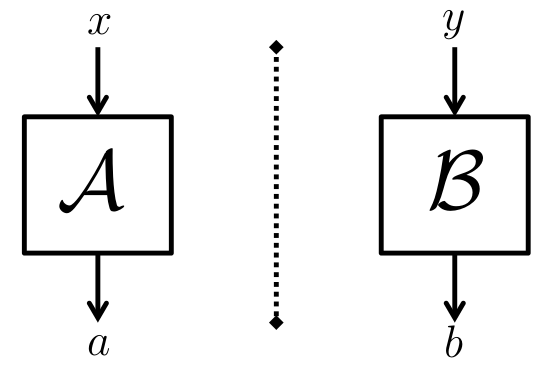
\includegraphics[scale=0.25]{BellGame.png}\\}
    \only<3>{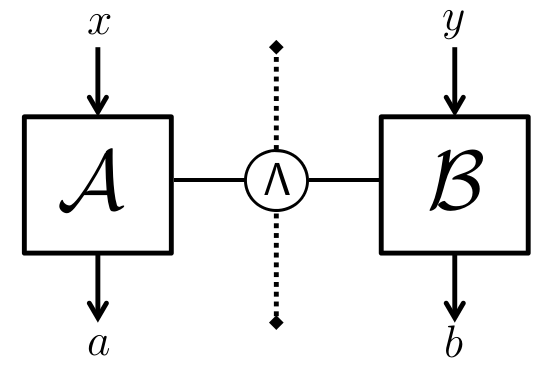
\includegraphics[scale=0.25]{BellGameWithLambda.png}\\}
    \only<4>{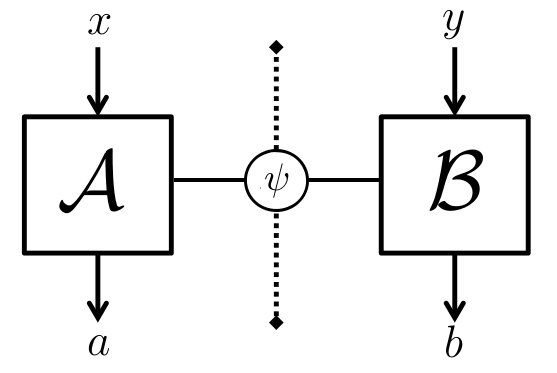
\includegraphics[scale=0.25]{BellGameWithPsi.png}\\}
    \only<5>{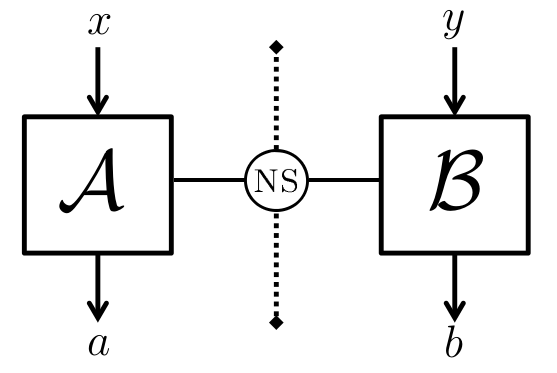
\includegraphics[scale=0.25]{BellGameWithNS.png}\\}
    \emph{What form can take $p(ab|xy)$?}
  \end{center}
  \pause
  \begin{itemize}
    \only<1-2>{\item Nothing more given : $p(ab|xy) = \alert{\mathcal{A}(a|x) \times \mathcal{B}(b|y)}$}
    \only<3>{\item Shared RV $\Lambda$ : $p(ab|xy) = \alert{\sum_{\lambda} \Lambda(\lambda)\mathcal{A}_{\lambda}(a|x)\mathcal{B}_{\lambda}(b|y)}$}
    \only<4>{\item Shared quantum entangled $\psi$ : $p(ab|xy) = \alert{\bra{\psi} \mathcal{A}^x_a \otimes \mathcal{B}^y_b \ket{\psi}}$}
    \only<5>{\item \textbf{Any $p(ab|xy)$ s.t.} \alert{$p(a|xy)=p(a|xy')$} and \alert{$p(b|xy)=p(b|x'y)$}}
  \end{itemize}
    
\end{frame}

\begin{frame}{The non-signaling assisted MAC coding problem}
      \only<1>{
  \begin{center}
  \begin{tikzpicture}[auto, node distance=2cm,>=latex']
    \node [input, name=i1] {};
    \node [block, right of=i1] (e1) {$e_1$};
    \node [bigblock, below right of=e1] (W) {$W$};
    \node [block, below left of=W] (e2) {$e_2$};
    \node [input, left of=e2, name=i2] {};
        

    \node [block, right of=W] (d) {$d$};

    \draw [->] (e1) -- node[name=x1] {$x_1$} (W);
    \draw [->] (e2) -- node[name=x2] {$x_2$} (W);
    \draw [->] (W) -- node[name=y] {$y$} (d);
    \node [output, right of=d] (j1j2) {};

    \draw [draw,->] (i1) -- node {$i_1$} (e1);
    \draw [draw,->] (i2) -- node {$i_2$} (e2);
    \draw [draw,->] (d) -- node {$(j_1,j_2)$} (j1j2);
  \end{tikzpicture}
  \end{center}
      }
      \only<2-3>{
  \begin{center}
  \begin{tikzpicture}[auto, node distance=2cm,>=latex']
    \node [input, name=i1] {};
    \node [input, name=i2] {};
    \node [Bigblock, below of=i2] (P) {\only<2>{$e_1\ \ \ \ \ \ e_2\ \ \ \ \ \ d$}\only<3>{\alert{$P(x_1x_2(j_1j_2)|i_1i_2y)$}}};

    
    \only<2>{\draw (P.120) -- (P.240);}\only<3>{\draw[dotted] (P.120) -- (P.240);}
    \only<2>{\draw (P.60) -- (P.300);}\only<3>{\draw[dotted] (P.60) -- (P.300);}


    \draw [<-] (P.130) -- node {$i_1$} +(0pt,1cm);
    \draw [<-] (P.90) -- node {$i_2$} +(0pt,1cm);
    \coordinate (ybis) at ($ (P.50) + (0pt,1.65cm) $);
    \draw [<-] (P.50) -- (ybis);
    \coordinate (x1) at ($ (P.230)+(0pt,-0.5cm) $);
    \draw [-] (P.230) -- (x1);
    \coordinate (x2) at ($ (P.270)+(0pt,-1cm) $);
    \draw [-] (P.270) -- (x2);
    \draw [->] (P.310) -- node {$(j_1,j_2)$} +(0pt,-1cm);

    \node [left of=P] (A) {};
    \node [bigblock, left of=A] (W) {$W$};
    \coordinate (x1bis) at ($ (x1)+(-3.65cm,0pt) $);
    \coordinate (x2bis) at ($ (x2)+(-3.65cm,0pt) $);
    \draw [-] (x1) -- node {$x_1$} (x1bis);
    \draw [-] (x2) -- node {$x_2$} (x2bis);
    \draw [->] (x1bis) -- (W.234);
    \draw [->] (x2bis) -- (W.303);
    \coordinate (y) at ($ (W.north)+(0pt,2cm) $) ;
    \draw (W.north) -- (y);
    \draw (y) -- node {$y$} (ybis);
  \end{tikzpicture}
  \end{center}
  }
\end{frame}

\begin{frame}{$\mathrm{S}^{\mathrm{NS}}(W,k_1,k_2)$ written as a \emph{linear} program}
\begin{equation*}
  \begin{aligned}
    &&\underset{P}{\maxi} &&& \frac{1}{k_1k_2} \sum_{x_1,x_2,y,i_1,i_2} W(y|x_1x_2)\alert{P(x_1x_2(i_1i_2)|i_1i_2y)}\\
    &&\st &&& \sum_{x_1} P(x_1x_2(j_1j_2)|i_1i_2y) = \sum_{x_1} P(x_1x_2(j_1j_2)|i_1'i_2y)\\
    &&&&& \sum_{x_2} P(x_1x_2(j_1j_2)|i_1i_2y) = \sum_{x_2} P(x_1x_2(j_1j_2)|i_1i_2'y)\\
    &&&&& \sum_{j_1j_2} P(x_1x_2(j_1j_2)|i_1i_2y) = \sum_{j_1j_2} P(x_1x_2(j_1j_2)|i_1i_2y')\\
    &&&&& \sum_{x_1,x_2,j_1,j_2} P(x_1x_2(j_1j_2)|i_1i_2y) = 1\\
    &&&&& P(x_1x_2(j_1j_2)|i_1i_2y) \geq 0
  \end{aligned}
\end{equation*}
\end{frame}

%\begin{frame}{A first step towards simplification}
%  \begin{itemize}
%  \item An equivalent program can be obtained with
%    \only<1>{
%      \begin{equation*}
%        \begin{aligned}
%          &r_{x_1,x_2,y} := \sum_{i_1,i_2} P(x_1x_2(i_1i_2)|i_1i_2y) \ ,\\ &r^1_{x_1,x_2,y} := \sum_{j_1,i_1,i_2} P(x_1x_2(j_1i_2)|i_1i_2y) \ ,\\
%          &r^2_{x_1,x_2,y} := \sum_{j_2,i_1,i_2} P(x_1x_2(i_1j_2)|i_1i_2y) \ ,\\ &p_{x_1,x_2} := \sum_{j_1,j_2,i_1,i_2} P(x_1x_2(j_1j_2)|i_1i_2y) \ . \\
%        \end{aligned}
%    \end{equation*}}
%    \only<2>{
%      \begin{equation*}
%        \begin{aligned}
%          P(x_1x_2(i_1i_2)|i_1i_2y) &:= \frac{r_{x_1,x_2,y}}{k_1k_2} \ ,\\
%          P(x_1x_2(j_1i_2)|i_1i_2y) &:= \frac{r^1_{x_1,x_2,y} - r_{x_1,x_2,y}}{k_1k_2(k_1-1)} \ ,\\
%          P(x_1x_2(i_1j_2)|i_1i_2y) &:= \frac{r^2_{x_1,x_2,y} - r_{x_1,x_2,y}}{k_1k_2(k_2-1)} \ ,\\
%          P(x_1x_2(j_1j_2)|i_1i_2y) &:= \frac{p_{x_1,x_2} -  r^1_{x_1,x_2,y} - r^2_{x_1,x_2,y} + r_{x_1,x_2,y}}{k_1k_2(k_1-1)(k_2-1)}.
%        \end{aligned}
%      \end{equation*}
%      }
%  \end{itemize}
%\end{frame}

%\begin{frame}{$\mathrm{S}^{\mathrm{NS}}(W,k_1,k_2)$ simplified linear program}
%  \begin{equation*}
%  \begin{aligned}
%    &&\underset{r,r^1,r^2,p}{\maxi} &&& \frac{1}{k_1k_2} \sum_{x_1,x_2,y} W(y|x_1x_2)r_{x_1,x_2,y}\\
%    &&\st &&& \sum_{x_1,x_2} r_{x_1,x_2,y} = 1\\
%    &&&&& \sum_{x_1} r^1_{x_1,x_2,y} = k_1 \sum_{x_1} r_{x_1,x_2,y}, \sum_{x_2} r^2_{x_1,x_2,y} = k_2 \sum_{x_2} r_{x_1,x_2,y}\\
%    &&&&& \sum_{x_1} p_{x_1,x_2} = k_1 \sum_{x_1} r^2_{x_1,x_2,y},  \sum_{x_2} p_{x_1,x_2} = k_2 \sum_{x_2} r^1_{x_1,x_2,y}\\
%    &&&&& 0 \leq r_{x_1,x_2,y} \leq r^1_{x_1,x_2,y},r^2_{x_1,x_2,y} \leq p_{x_1,x_2}\\
%    &&&&& p_{x_1,x_2} -  r^1_{x_1,x_2,y} - r^2_{x_1,x_2,y} + r_{x_1,x_2,y} \geq 0
%  \end{aligned}
%  \end{equation*}
%\end{frame}

\begin{frame}{Non-signaling assisted capacity regions}
    \begin{defi}[Capacity region \only<1>{$\mathcal{C}^{\mathrm{NS}}(W)$}\only<2-3>{$\mathcal{C}^{\mathrm{NS}}_0(W)$} of a MAC $W$]
  \label{defi:capacity}
  $(R_1,R_2)$ achievable with\only<2-3>{\alert{ zero-error} and} non-signaling assistance if:
  \only<1>{\[ \underset{n \rightarrow +\infty}{\lim} \mathrm{S}^{\mathrm{NS}}(W^{\otimes n},\ceil{2^{R_1n}},\ceil{2^{R_2n}}) = 1 \ . \]
    $\mathcal{C}^{\mathrm{NS}}(W)$ is the set of all achievable rate pairs with non-signaling assistance.}
  \only<2-3>{\[ \alert{\exists n_0  \in \mathbb{N}^*, \forall n \geq n_0,} \mathrm{S}^{\mathrm{NS}}(W^{\otimes n},\ceil{2^{R_1n}},\ceil{2^{R_2n}}) = 1 \ . \color{white}{\underset{n \rightarrow +\infty}{\lim}}  \]
  $\mathcal{C}^{\mathrm{NS}}_0(W)$ is the set of all achievable rate pairs with \alert{zero-error} and non-signaling assistance.}
    \end{defi}
    \pause
    \pause
    \begin{prop}[Lower bounds on $\mathcal{C}^{\mathrm{NS}}_0(W)$]
      For any MAC $W$ and integers $k_1,k_2,n$:
      \begin{equation*}
        \begin{aligned}
          \mathrm{S}^{\mathrm{NS}}(W^{\otimes n},k_1,k_2) = 1 \implies \left(\frac{\log_2(k_1)}{n},\frac{\log_2(k_2)}{n}\right) &\in \mathcal{C}^{\mathrm{NS}}_0(W)\\
          &\subseteq \mathcal{C}^{\mathrm{NS}} (W) \ .
        \end{aligned}
      \end{equation*}
    \end{prop}
\end{frame}


\begin{frame}{Symmetrization and main result}
  \begin{itemize}
  \item $W^{\otimes n} := n$ independent copies of $W$.
  \item LP size $\Omega(|W|^n)$: hard to compute $\mathrm{S}^{\mathrm{NS}}(W^{\otimes n},k_1,k_2)$ \emph{a priori}.
  \end{itemize}
    \pause

    \begin{theo}
        $\mathrm{S}^{\mathrm{NS}}(W^{\otimes n},k_1,k_2)$ is the solution of a linear program of size bounded by $O\left(n^{|\mathcal{X}_1|\cdot|\mathcal{X}_2 |\cdot|\mathcal{Y}|-1}\right)$: it can be computed in time $\text{poly}(n)$.
    \end{theo}
    
    \pause
    \bigskip
    
    \begin{itemize}
    \item Formally, for any MAC $W$ invariant under the action of a group $G$, $\mathrm{S}^{\mathrm{NS}}(W,k_1,k_2)$ solution of a linear program of polynomial size in the number of orbits of that action.
    \item Apply to $W^{\otimes n}$ and $G=S_n$, the group of permutations on $[n]$.
    \end{itemize}
\end{frame}

%%%%%%%%%%%%%%%%%%%%%%%%%%%%%%%%%%%%%%%%%%
\section{The Binary Adder Channel}
%%%%%%%%%%%%%%%%%%%%%%%%%%%%%%%%%%%%%%%%%%
\begin{frame}{The Binary Adder Channel}
  \begin{itemize}
  \item For bits $x_1,x_2$, $W_{\text{BAC}}(x_1x_2) := x_1 + x_2$ (deterministic):
    \[ W_{\text{BAC}}(00) = 0; \alert{W_{\text{BAC}}(01) = W_{\text{BAC}}(10)=1}; W_{\text{BAC}}(11) = 2 \ . \]
    
    \pause
  \item Thanks to \cite{Liao73,Ahlswede73} and their general single-letter formula, its classical capacity region is known:
    \[ \mathcal{C}(W_{\text{BAC}}) = \left\{(R_1, R_2) : R_1 \leq 1, R_2 \leq 1, R_1 + R_2 \leq 3/2\right\} \ .\]

    \pause

  \item Only lower bounds known on its zero-error capacity region.
  \item \cite{MO05}: $\log_2(240/6) \simeq 1.3178$ best achievable sum-rate with zero-error so far.
  \end{itemize}
\end{frame}


\begin{frame}{Numerical results for $W_{\text{BAC}}$}
    \begin{center}
      \begin{tikzpicture}
        \begin{axis}[
          xmin = 0, xmax = 1.05,
          ymin = 0, ymax = 1.05,
          xtick distance = 0.25,
          ytick distance = 0.25,
          grid = both,
          width = 0.6\textwidth,
          height = 0.6\textwidth,
          legend cell align = {left},
          legend pos = outer north east,
          ylabel=$R_2$,
          xlabel=$R_1$,
          ]
          \addplot[
          domain = 0.25:0.33,
          darkgray,
          densely dashed,
        ] {(1 + -(2*\x)*ln(2*\x)/ln(2))-(1-2*\x)*ln(1-2*\x)/ln(2))/2};
          \draw[
            domain=0.25:0.33,
            variable=\y,
            darkgray,
            densely dashed
          ] plot({(1 + -(2*\y)*ln(2*\y)/ln(2))-(1-2*\y)*ln(1-2*\y)/ln(2))/2},\y);
        \addplot[
          darkgray,
          densely dashed,
        ]  coordinates {(0,1) (0.25,1)};
        \addplot[
          darkgray,
          densely dashed,
        ]  coordinates {(1,0) (1,0.25)}; 
        \addplot[
          thick,
          dashed,
          black,
        ] coordinates {(0,1) (0.5,1) (1,0.5) (1,0)};
        \addplot[
          densely dashed,
          darkgray,
          mark = star,
        ] coordinates {(0.33, 0.962409352487) (0.43425,0.86873) (0.59749375012,0.720321349148) (0.720321349148,0.59749375012) (0.86873,0.43425) (0.962409352487,0.33)};
        \only<2-4>{\addplot[
          domain = 0:1,
          brown,
          mark = triangle,
        ] table[x=R1,y=R2,col sep=comma] {Data_BAC/ZEBorder2.csv};}
         \only<3-4>{\addplot[
          domain = 0:1,
          red,
          mark = o,
        ] table[x=R1,y=R2,col sep=comma] {Data_BAC/ZEBorder3.csv};}
         \only<4>{\addplot[
          domain = 0:1,
          blue,
          mark = x,
        ] table[x=R1,y=R2,col sep=comma] {Data_BAC/ZEBorder6.csv};}

         \legend{,,,Classical CR, Best ZE Lower Bounds, \only<2-4>{NS ZE CR  for $2$ copies}, \only<3-4>{NS ZE CR  for $3$ copies}, \only<4>{NS ZE CR for $6$ copies}}
        \end{axis}
      \end{tikzpicture}
    \end{center}
\end{frame}


\begin{frame}{Handling errors with concatenated codes}
  \begin{center}
  \begin{tikzpicture}[auto, node distance=2cm,>=latex']
    \node [input, name=i1] {};
    \node [input, name=i2] {};
    \node [Bigblock, below of=i2] (P) {$P(x_1x_2j|i_1i_2y)$};

    \draw [<-] (P.130) -- node {$i_1$} +(0pt,1cm);
    \draw [<-] (P.90) -- node {$i_2$} +(0pt,1cm);
    \coordinate (ybis) at ($ (P.50) + (0pt,1.65cm) $);
    \draw [<-] (P.50) -- (ybis);
    \coordinate (x1) at ($ (P.230)+(0pt,-0.5cm) $);
    \draw [-] (P.230) -- (x1);
    \coordinate (x2) at ($ (P.270)+(0pt,-1cm) $);
    \draw [-] (P.270) -- (x2);
    \draw [->] (P.310) -- node {$j$} +(0pt,-1cm);

    \node [left of=P] (A) {};
    \node [bigblock, left of=A] (W) {$W$};
    \coordinate (x1bis) at ($ (x1)+(-3.65cm,0pt) $);
    \coordinate (x2bis) at ($ (x2)+(-3.65cm,0pt) $);
    \draw [-] (x1) -- node {$x_1$} (x1bis);
    \draw [-] (x2) -- node {$x_2$} (x2bis);
    \draw [->] (x1bis) -- (W.234);
    \draw [->] (x2bis) -- (W.303);
    \coordinate (y) at ($ (W.north)+(0pt,2cm) $) ;
    \draw (W.north) -- (y);
    \draw (y) -- node {$y$} (ybis);

    \node [left of=W] (Equal) {$:=$};
    \node [bigblock, left of=Equal] (WP) {$W[P]$};

    \draw [<-] (WP.130) -- node {$i_1$} +(0pt,1cm);
    \draw [<-] (WP.50) -- node {$i_2$} +(0pt,1cm);
    \draw [->] (WP.270) -- node {$j$} +(0pt,-1cm);
    
  \end{tikzpicture}
\end{center}
\end{frame}

\begin{frame}{Method to find lower bounds on $\mathcal{C}^{\mathrm{NS}}(W)$}
  \begin{itemize}
  \item Applying MAC capacity single-letter formula on $W^{\otimes n }[P]$ gives an achievable non-signaling assisted rate pair for $W$:
    
    \pause
    
    \begin{prop}
      %For any $(k_1,k_2)$-non-signaling code $P$ for $W^{\otimes n}$ and product distribution $q_1,q_2$ on $[k_1],[k_2]$,
      The following $(R_1,R_2)$ are in $\mathcal{C}^{\mathrm{NS}}(W)$:
  \[ R_1 \leq \frac{I(I_1:J|I_2)}{n}\ ,\ R_2 \leq \frac{I(I_2:J|I_1)}{n}\ ,\ R_1+R_2 \leq \frac{I((I_1,I_2):J)}{n} \ ,\]
  for inputs $(I_1,I_2) \sim q_1 \times q_2$, and $J$ outcome of $W^{\otimes n }[P]$.
    \end{prop}
    
    \pause
    \bigskip
  
  \item Focus on noisy BAC $W_{\text{BAC},\varepsilon,\varepsilon}$: bit flip error of $\varepsilon$ on each input.
  \end{itemize}
\end{frame}

\begin{frame}{Numerical results for $W_{\text{BAC},\varepsilon,\varepsilon}$ with $\varepsilon = 10^{-3}$}
  \begin{center}
      \begin{tikzpicture}
        \begin{axis}[
          xmin = 0, xmax = 1.05,
          ymin = 0, ymax = 1.05,
          xtick distance = 0.25,
          ytick distance = 0.25,
          grid = both,
          width = 0.6\textwidth,
          height = 0.6\textwidth,
          legend cell align = {left},
          legend pos = outer north east,
          ylabel=$R_2$,
          xlabel=$R_1$,
        ]
        \addplot[
          thick,
          dashed,
          black,
        ] coordinates {(0,1) (0.49429612113126953,0.983898049082558) (0.983898049082558, 0.49429612113126953) (1,0)};
        \addplot[
          red,
          mark = o,
          thick,
        ] coordinates {(0,0)};
        \only<2-3>{\addplot[
          domain = 0:1,
          brown,
          mark = triangle,
        ] table[x=R1,y=R2,col sep=comma] {Data_Capacity_BACwithSmallBitFlipNoise/Capacity3.csv};}
        \only<3>{\addplot[
          domain = 0:1,
          blue,
          mark = x,
        ] table[x=R1,y=R2,col sep=comma] {Data_Capacity_BACwithSmallBitFlipNoise/Capacity5.csv};}
        \legend{Classical CR, NS with zero-error CR, NS Rates for $3$ copies, NS Rates for $5$ copies}
        \end{axis}
      \end{tikzpicture}
  \end{center}
\end{frame}


\appendix
%%%%%%%%%%%%%%%%%%%%%%%%%%%%%%%%%%%%%%%%%%
\section{Conclusion and open problems}
\begin{frame}{Conclusion and open problems}
  \begin{enumerate}
    \item \underline{What was found:}
      \begin{itemize}
      \item Efficient linear program computing $\mathrm{S}^{\mathrm{NS}}(W^{\otimes n},k_1,k_2)$.
        \pause
      \item Applied to the BAC, a sum-rate of $\frac{\log_2(72)}{4} \simeq 1.5425$ can be reached with zero-error and non-signaling assistance, beating the classical sum-rate of $\frac{3}{2}$.
        \pause
      \item Handle noisy channels through concatenated codes:\\
        Previous gap persists for noisy BAC.
      \end{itemize}
      \pause
      \bigskip
      \item \underline{Open problems:}
        \begin{itemize}
  \item Suggests that quantum entanglement may increase the capacity of such channels: still open for the BAC !
    \pause
  \item How are linked $\mathcal{C}^{\mathrm{NS}}(W)$ and the set of $(R_1,R_2)$ such that:
  \[ R_1 \leq I(X_1:Y|X_2)\ ,\ R_2 \leq I(X_2:Y|X_1)\ ,\ R_1+R_2 \leq I((X_1X_2):Y)\]
  for inputs $(X_1,X_2) \in \mathcal{X}_1 \times \mathcal{X}_2$ following \alert{any input law $P_{X_1X_2}$}?
        \end{itemize}
  \end{enumerate}
\end{frame}

\begin{frame}
  \begin{center}
    \emph{\huge{Thank you for listening!}}
    \end{center}
\end{frame}

%%%%%%%%%%%%%%%%%%%%%%%%%%%%%%%%%%%%%%%%%%
\section{Bibliography}
\begin{frame}[allowframebreaks]{Bibliography}
  \bibliographystyle{apalike}
  \bibliography{MAC_NS}
\end{frame}
%%%%%%%%%%%%%%%%%%%%%%%%%%%%%%%%%%%%%%%%%%

%%%%%%%%%%%%%%%%%%%%%%%%%%%%%%%%%%%%%%%%%%
\end{document}
%%%%%%%%%%%%%%%%%%%%%%%%%%%%%%%%%%%%%%%%%%
